%! Author = Yan Wittmann


\chapter{Projektbericht} \label{ch:projektbericht}

In der Einleitung (Kapitel\ \ref{sec:projektbericht-projektziel}) wird zunächst auf die Abteilung im Unternehmen, die aktuelle Situation und die Ziele für das Projektsemester eingegangen.
Bei den darauf folgenden Grundlagen (Kapitel\ \ref{sec:projektbericht-grundlagen}) werden die relevanten Themen, Begriffe und Standards erklärt.


\section{Einleitung, Problemstellungen und Projektziel} \label{sec:projektbericht-projektziel}

Die für dieses Praktikum relevante Abteilung in der {\metaeffekt} stellt ein automatisiertes Vulnerability Monitoring her und integriert es bei diversen Kunden, deren Wünsche und Anforderungen priorisiert in die Systeme zurückgeführt werden.
Das Vulnerability Monitoring wird intern durch eine Aneinanderreihung von Prozessschritten modelliert, die auch als \qt{Inventory Enrichment Pipeline} bezeichnet wird.
Die Prozessschritte erhalten jeweils ein Software-Inventar als Eingabe, welches sie auf eine bestimmte definierte Weise modifizieren und für den nächsten Schritt bereitstellen, sodass ein Inventar, das alle Schritte durchlaufen hat, alle nötigen Schwachstell-Informationen angereichert bekommen hat.
Auf diese Pipeline wird im Kapitel\ \ref{subsec:projektbericht-grundlagen-vulnerability-monitoring} kurz eingegangen, sie soll allerdings nicht Hauptbestandteil dieses Berichts sein und dient nur zur besseren Einordnung der anderen Prozesse.

In dem Praktikum liegt der Schwerpunkt vor allem auf dem CVSS-Standard\textsuperscript{\ref{subsec:projektbericht-grundlagen-cvss}}, insbesondere in der Verbesserung unseres Supports für neuere Versionen dieses und in konzeptionelle Änderungen, wie das System mit diesen umgehen sollte.
Konkret geht es um die folgenden Punkte:

\begin{smitemize}
    \item Die Veröffentlichung der neuesten Version 4.0 des CVSS-Standards am 31.\ Oktober 2023\footnote{\url{https://www.first.org/cvss/v4-0/}} hat bereits und wird über die nächsten Monate zur Folge haben, dass CVSS-Vektoren der Version 4.0 für Schwachstellen in den öffentlichen Datenbanken auftauchen werden, die die {\metaeffekt} in der Lage sein muss, zu parsen und zu berechnen.
    Es ist dazu also notwendig, die aktuelle Implementierung der Versionen 2.0 und 3.1 um die vierte zu erweitern.
    Zu der Implementierung der Berechnungslogik muss sie auch noch in die vorhandenen Systeme integriert und die Theorie dahinter verstanden werden, auch damit man gegenüber Kunden aussagekräftig die Unterschiede und die Vorteile begründen kann.
    \item Über die Monate vor dem Praktikum ist es bereits immer deutlicher geworden, dass das Datenmodell hinter dem Vulnerability Monitoring fast komplett neu geschrieben werden muss, um neue Anforderungen und Erkenntnisse effizient und korrekt unterstützen zu können.
    Die relevante Anforderung an das Datenmodell ist es, die Art und Weise, wie die CVSS-Vektoren abzulegen und verarbeitet werden, komplett neu zu planen und zu schreiben.
    Es wurde erkannt, dass meistens nicht nur ein CVSS-Vektor einer Quelle pro Schwachstelle (CVE, \ldots) vorhanden ist, sondern mehrere, die von mehreren Organisationen und Institutionen vergeben werden, da ihre Meinungen über den Schweregrad voneinander abweichen können.
    Bisher wird mit diesen zusätzlichen Vektoren nicht bewusst unterschiedlich umgegangen, es wird einfach der erste verarbeitet, der vorhanden ist.
    Um diese Situation zu verbessern, soll ein System eingeführt werden, das über die einzelnen Schritte der Inventory Enrichment Pipeline nur die Vektoren aggregiert und noch nicht verarbeitet oder berechnet.
    Erst zum Ende, wenn es darum geht die Reports (PDF, HTML) zu generieren, sollen die Vektoren ausgewählt, eventuell kombiniert und deren Scores berechnet werden.
    Bei dem Überarbeiten des Datenmodells muss also darauf geachtet werden, diese Anforderung zu unterstützen.
    Zudem muss ein CVSS-Selektor geschrieben werden, der die darzustellenden Vektoren berechnen kann.
    \item Zuletzt ging es noch um die Implementierung des CVSS-Standards in TypeScript, die Open Source gestellt werden sollte und mit einem Web-UI als online verfügbarer, interaktiver CVSS-Rechners verfügbar sein soll.
    Dieser soll dann aus den eigenen Reports verlinkt werden können.
    Der Grund hierfür ist simpel: Es gibt bisher keinen online CVSS-Rechner, der alle unsere Anforderungen erfüllt.
    Es gibt keinen Rechner, der alle Versionen zugleich unterstützt, keinen, der mehrere Vektoren gleichzeitig gut vergleichbar zulässt und leider haben viele der offiziellen Rechner auch Probleme, die URL-Parameter korrekt zu erkennen.
\end{smitemize}

In diesem Bericht wird ein Fokus auf die CVSS-seitigen Arbeiten im Unternehmen gelegt, da sie den Großteil des Semesters eingenommen haben.


% Grundlagen


\section{Grundlagen} \label{sec:projektbericht-grundlagen}

\subsection{Software-Inventare} \label{subsec:projektbericht-grundlagen-inventories}

Software-Inventare werden bei der {\metaeffekt} in einem eigens entwickelten, proprietären Format, schlicht \qt{Inventar} genannt, abgelegt.
Meist wird, um ein solches Inventar zu erhalten, ein ebenfalls eigens entwickelter Scanner verwendet, der ganze Dateisysteme nach Komponenten durchsucht und daraus ein Inventar generiert.
Um möglichst breiten Support zu bieten, gibt es allerdings nicht nur den Scanner, sondern auch diverse Konverter, mit denen Inventare von und zu Formaten wie CycloneDX SBOM\footnote{\url{https://cyclonedx.org/specification/overview}} oder SPDX\footnote{\url{https://spdx.dev}} umgewandelt werden können.

Diese Inventare können mehrere Kategorien an Daten enthalten: Software-Komponenten (\qt{Artefakte}), Schwachstell-Informationen, Security Advisories, Lizenzinformationen und einige weitere.

\subsection{NVD / NIST} \label{subsec:projektbericht-grundlagen-nvd-nist}

Software-Schwachstellen sind allgegenwärtig, jedes Softwareprodukt hat sie und meistens es ist nur eine Frage der Zeit, bis sie gefunden, veröffentlicht und im schlimmsten Fall ausgenutzt werden.
Die National Vulnerability Database (NVD)\footnote{\url{https://nvd.nist.gov}} des National Institute of Standards and Technology (NIST) der U.S.\ Regierung stellt mit ihrem CVE-System\textsuperscript{\ref{subsec:projektbericht-grundlagen-cve-cpe}} eine der primären Quellen für Schwachstell-Informationen für Forscher, Unternehmen und automatisierte Tools bereit.
Sobald eine neue Schwachstelle bekannt gegeben wird, nehmen sie diese in ihren Katalog an CVE mit auf, versehen sie mit CVSS- und Matching-Informationen über das CPE-System.
Damit ist die Schwachstelle für alle auf der Welt über eine API oder über ihr User Interface erreichbar und kann, falls ein Projekt betroffen ist, frühzeitig kontextualisiert bewertet werden.

\subsection{CVE / CPE} \label{subsec:projektbericht-grundlagen-cve-cpe}

\qt{CVE} ist ein von dem CVE Project eingeführtes System, das Schwachstellen in Software- und Hardwareprodukten eindeutig identifiziert und beschreibt.
Der Standard wird stark von der NVD des NIST unterstützt.
Im CVE-System bekommt jede Schwachstelle, die von einem Forscher oder einer Organisation gefunden und veröffentlicht wird, eine eindeutige ID von der Form \qt{CVE-YYYY-NNNN} zugewiesen, wobei \qt{YYYY} das Jahr der Veröffentlichung und \qt{NNNN} eine eindeutige, fortlaufende Nummer ist.
CVE definiert eine Schwachstelle als:

\begin{quote}
    A weakness in the computational logic (e.g., code) found in software and hardware components that, when exploited, results in a negative impact to confidentiality, integrity, or availability.
    Mitigation of the vulnerabilities in this context typically involves coding changes, but could also include specification changes or even specification deprecations (e.g., removal of affected protocols or functionality in their entirety).
    \cite{nvdVulnerabilityDefinition}
\end{quote}

Eine Schwachstelle ist also eine Schwäche, eine theoretische Angriffsfläche, die durch Ausnutzen negative Auswirkungen auf die Vertraulichkeit, Integrität oder Verfügbarkeit eines Systems hat.
Es soll kein CVE-Eintrag existieren, der keinen Einfluss auf die Vertraulichkeit, Integrität oder Verfügbarkeit eines Systems hat \cite{nvdVulnerabilityMetrics}.

Jeder CVE werden gewisse Metadaten zugeordnet, wie Beschreibungen, Referenzen und (potenziell mehrere) CVSS-Vektoren zur Bewertung des Schweregrads, aber auch \qt{CPE}s, die Aussagen über die betroffenen Produkte machen und automatisierte Zuordnungen erlauben.
Common Platform Enumeration (CPE) ist ein von der MITRE Corporation\footnote{\url{https://cpe.mitre.org/specification}} entwickeltes System, mit dem Soft- und Hardwareprodukte über den Hersteller, Produktnamen und Version eindeutig identifiziert werden können.
Die CPE Naming Specification Version 2.3 \cite[Seite 37, Kapitel 6.2]{NISTIR7695} definiert die Syntax eines CPE-Strings, in der mindestens \qt{part} (Komponenten-Typ), \qt{vendor} (Hersteller) und \qt{product} (Produkt) gesetzt sein müssen:

\code{cpe : 2.3 : part : vendor : product : version : update : edition}\newline\hphantom{\code{cpe}}\code{: language : sw_edition : target_sw : target_hw:other}

Auf dem NVD Dashboard\footnote{\url{https://nvd.nist.gov/general/nvd-dashboard}} ist gelistet, dass es am 08.03.2024 insgesamt 240899 eindeutige CVEs und 1261617 CPEs gibt.
Diese Zahl wächst exponentiell und zeigt, wie wichtig es ist, Schwachstellen automatisiert zu verarbeiten.

\subsection{CVSS} \label{subsec:projektbericht-grundlagen-cvss}

Das Common Vulnerability Scoring System (CVSS) wird in Version 4.0 \cite{CVSSv4.0Specification} vom FIRST\footnote{\url{https://www.first.org}} (Forum of Incident Response and Security Teams) als ein offener Standard für die Bewertung der Sicherheitsanfälligkeit von Software- und Hardwarekomponenten beschrieben.
Dieser Standard legt fest, wie sog\. CVSS-Vektoren, definiert als Sammlung von Schlüssel-Wert Paaren, zur möglichst objektiven Darstellung von Schwachstelleneigenschaften genutzt werden können.
Solche Vektoren können textuell als \code{CVSS:VERSION/KEY:VALUE/KEY:VALUE/...} formatiert werden, wobei jedes Wertepaar durch \qt{/} getrennt und mit \qt{CVSS:} gefolgt von der Vektor-Version beginnen muss.

Ein Beispiel für einen Basisvektor in Version 3.1, der einen mittleren Schweregrad (\qt{Medium}) mit einem Score von 6.0 darstellt, kann folgendermaßen aussehen: \code{CVSS:3.1/AV:L/AC:L/PR:H/UI:N/S:U/C:H/I:H/A:N}.
Allgemein reichen die Scores, die aus diesen Vektoren berechnet werden, von 0 bis 10 und ordnen die Schwachstellen in die Kategorien \qt{Low}, \qt{Medium}, \qt{High} und \qt{Critical} ein, wobei höhere Werte eine dringendere Bewertung erfordern.
Diese Berechnungen lassen sich leicht mit Online-Rechnern\footnote{\url{https://metaeffekt.com/security/cvss/calculator}} oder Software-Tools, verfügbar in allen populären Programmiersprachen, durchführen.

Die versionsabhängigen Metriken der Vektoren ordnen jeweils eine Charakteristik einer Schwachstelle einem Wert zu.
So steht beispielsweise \code{AV:L} für einen \qt{Attack Vector} mit dem Wert \qt{Local}, was die räumliche Nähe beschreibt, die ein Angreifer benötigt, um die Schwachstelle auszunutzen.
Andere Werte wie \qt{Network} (aus dem Internet ausnutzbar, höchster Schweregrad), \qt{Adjacent Network} oder \qt{Physical} (physikalischer Zugang benötigt, am weigsten schlimm) spezifizieren weitere Angriffsszenarien für diese Metrik.

Zusätzlich zu den allgemeinen, umgebungsunabhängigen Basismetriken, die von den Herausgebern der Schwachstelleninformationen festgelegt werden, gibt es noch die \qt{Temporal}/\qt{Threat}- und \qt{Environmental}-Metriken.
Diese Metriken reflektieren die spezifische Umgebung und den Kontext, in dem eine Schwachstelle existiert, und werden in betroffenen Projekten von den Anwendern kontextabhängig gesetzt.
Damit erlaubt es CVSS, eine initiale, kontextunabhängige Bewertung eines Systems, und durch Hinzufügen von Kontextinformationen auch eine kontextualisierte Sicht auf das System zu erhalten.
Einer Schwachstelle können von verschiedenen Parteien potenziell mehrere, unterschiedliche Vektoren zugeordnet werden, dieser Aspekt wird später wichtig.

\subsection{Automatisiertes Vulnerability Monitoring} \label{subsec:projektbericht-grundlagen-vulnerability-monitoring}

Das bei der {\metaeffekt} eingesetzte automatisierte Vulnerability Monitoring, hat das Ziel, für ein gegebenes Software-Inventar nicht nur die relevanten Schwachstellen (\qt{Vulnerabilities}) zu identifizieren, sondern auch zugehörige Ratgeber (\qt{Security Advisories}) als Hilfestellung zu der darauf folgenden manuellen Bewertung bereitzustellen.
Der Prozess, dargestellt in Grafik \ref{fig:vulnerability-monitoring-overview-figure}, in zwei Hauptphasen mit mehreren Unterschritten gegliedert, wird im Folgenden beschrieben.
Als Eingabe dient in jedem Fall ein Inventar gefüllt mit einer Liste an Software-Komponenten und deren Metadaten, wie Version, Quelle und Ökosystem-spezifischen Informationen.

Der erste Prozessschritt ist die Identifikation von Schwachstellen und wird getrennt voneinander auf alle Komponenten im Inventar angewandt.
Die in unserem Prozess verwendeten externen Schwachstellendatenbanken nutzen abstrahierte Darstellungen von Produkten und Software-Komponenten für ihre internen Verweise zwischen Produkten und Schwachstellen.
Beispielsweise verwendet die NVD CPEs (siehe Kapitel \ref{subsec:projektbericht-grundlagen-cve-cpe}), GitHub Security Advisories\footnote{\url{https://github.com/advisories}} folgen dem OSV-Schema\footnote{\url{https://osv.dev}} mit Ökosystem-abhängigen Informationen, und Microsoft (MSRC)\footnote{\url{https://msrc.microsoft.com/update-guide}} arbeitet mit numerischen Identifikatoren, die nur durch Download und Extraktion aller monatlichen Zusammenfassungen über ihre API zugänglich sind.
Die Zuordnung unserer realen Komponenten zu diesen abstrahierten Produkten stellt daher immer eine Herausforderung dar.
Unser Vulnerability Monitoring setzt verschiedene Algorithmen ein, um diese Zuordnungen so weit wie möglich automatisch vorzunehmen, was jedoch nicht immer fehlerfrei gelingt.
Falsch positive und falsch negative Ergebnisse erfordern dann eine manuelle Korrektur durch einen gepflegten Datensatz (\qt{Korrelationsdaten}), was einen erheblichen Zeitaufwand bedeutet.

Wenn dieser Schritt erfolgreich abgeschlossen ist, können Abfragen an die jeweiligen Datenbanken gestartet werden, um Schwachstellen durch Produkt- und Versionsabgleichen zu identifizieren.
Dieses Zwischeninventar mit Schwachstellinformationen kann bereits für Berichte genutzt werden, jedoch wird meistens ein weiterer Schritt dahinter geschaltet:
Weitere Abfragen an einen größeren Satz an Datenbanken werden gestartet, um zu den gefundenen Schwachstellen entsprechende Ratgeber zuzuordnen.
Diese Abfragen sind in der Regel einfacher, da die Ratgeber-Einträge meistens direkt auf die betroffenen Schwachstellen-IDs Bezug nehmen.
Das Ergebnisinventar kann dann als Grundlage für die Erstellung von Reports und Statistiken benutzt werden.

\begin{figure}[htbp] % here, top, bottom, separate page
    \centering
    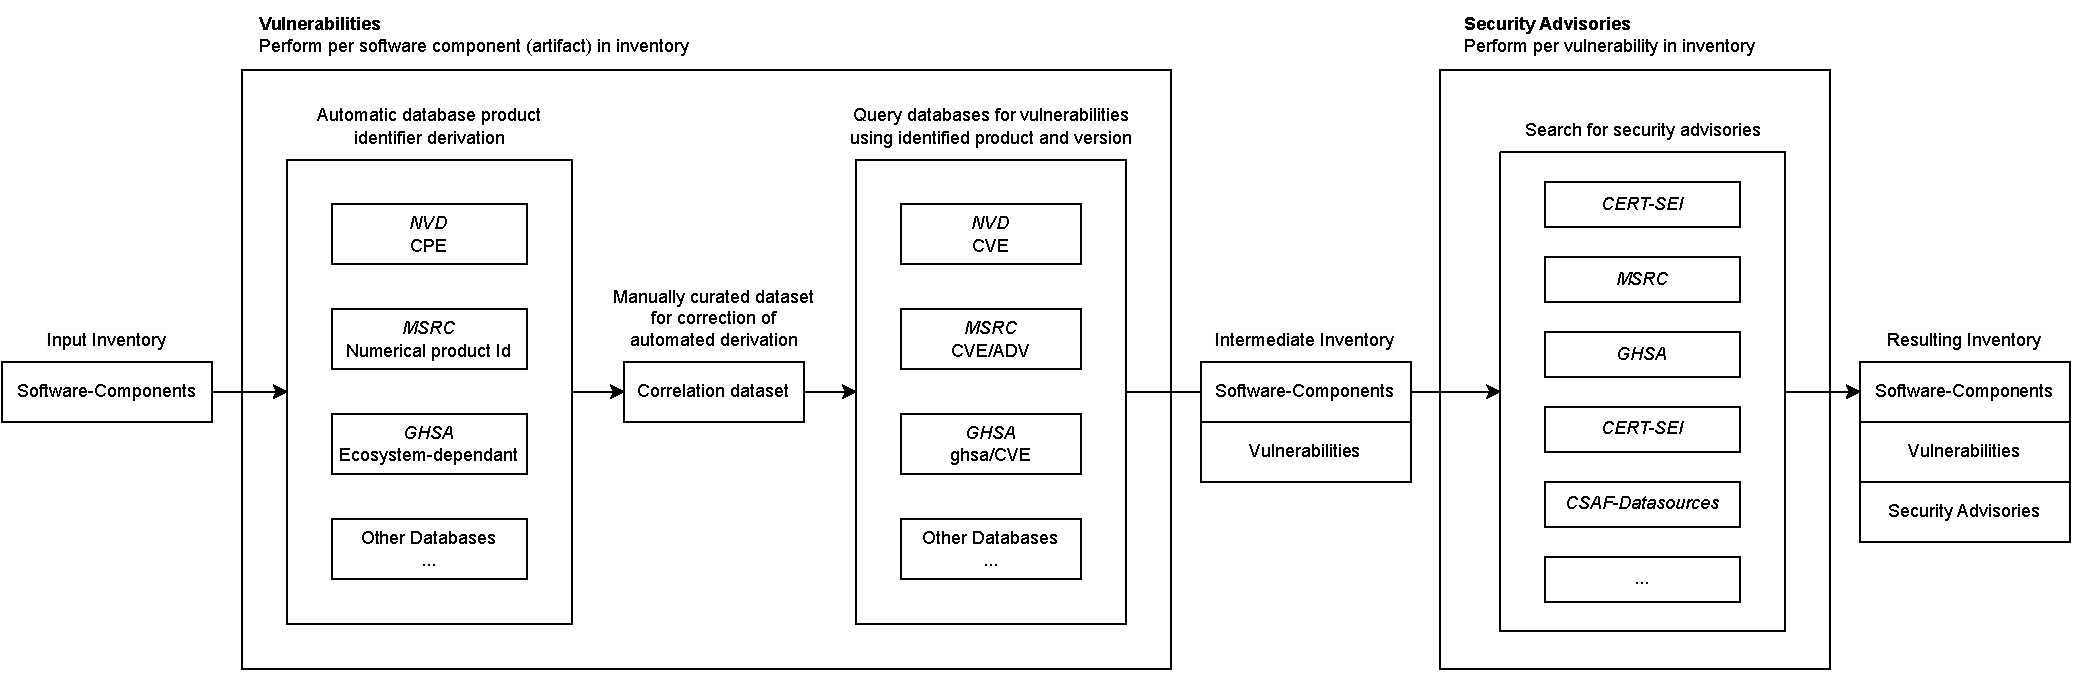
\includegraphics[width=1\textwidth, keepaspectratio]{res/grafiken/vulnerability-monitoring-overview}
    \caption{Schwachstellsuche mit einem Software-Inventar}
    \label{fig:vulnerability-monitoring-overview-figure}
\end{figure}

\subsection{Vulnerability Assessment} \label{subsec:projektbericht-grundlagen-vulnerability-assessment}
